\documentclass[12pt]{article}

\usepackage{scicite,times,graphicx,float,hyperref}
\usepackage[skip=0pt]{caption}
\usepackage[utf8]{inputenc}
\usepackage{enumitem}
\usepackage{booktabs}

%%%%%%%%%%%%%%%%%%%%%%%%%%%%%%%%%%%%%%%%%%%%%%%%%%%%%%%%%%%%%%%%%%%%%%%%%%% PREAMBLE %%%%%%%%%%%%%%%%%%%%%%%%%%%%%%%%%%%%%%%%%%%%%%%%%%%%%%%%%%%%%%%%%%%%%%%%%%%

\topmargin -1.0cm
\oddsidemargin 0.0cm 
\textwidth 16cm 
\textheight 23cm
\footskip 1.0cm

\newenvironment{sciabstract}{%
\begin{quote} \bf}
{\end{quote}}

\newcounter{lastnote}
\newenvironment{scilastnote}{%
  \setcounter{lastnote}{\value{enumiv}}%
  \addtocounter{lastnote}{+1}%
  \begin{list}%
  {\arabic{lastnote}.}
  {\setlength{\leftmargin}{.22in}}
  {\setlength{\labelsep}{.5em}}
}
{\end{list}}

\title{Final Report on:\\Pretix Cluster Deployment \& Management} 

\author
{Filipe Pires [85122], João Alegria [85048]\\
\\
Computational Infrastructures Management\\
\normalsize{Department of Electronics, Telecommunications and Informatics}\\
\normalsize{University of Aveiro}\\
} 

\date{\today{}}

%%%%%%%%%%%%%%%%%%%%%%%%%%%%%%%%%%%%%%%%%%%%%%%%%%%%%%%%%%%%%%%%%%%%%%%%%%%% REPORT %%%%%%%%%%%%%%%%%%%%%%%%%%%%%%%%%%%%%%%%%%%%%%%%%%%%%%%%%%%%%%%%%%%%%%%%%%%%

\begin{document} 

\baselineskip18pt

\maketitle 

\section*{Introduction} \label{introduction} %%%%%%%%%%%%%%%%%%%%%%%%%%%%%%%%%%%%%%%%%%%%%%%%%%%%%%%%%%%%%%%%%%%%%%%%%%%%%%%%%%%%%%%%%%%%%%%%%%%%%%%%%%%%%%%%%%%

This report aims to describe the work developed for the final phase of the practical assignment of the discipline of Computational Infrastructures 
Management \cite{assign} from the Msc. degree in Informatics Engineering of the University of Aveiro at the Department of Electronics, Telecommunications and 
Informatics.
It is assumed that the reader has knowledge about the previous report, and it is here included:
the characterization of the service level agreements for each service;
the description of the load balancing mechanisms amongst software components;
the redundancy strategy;
the listing of metrics and computational resources monitored, along with the respective defined alarms;
and other relevant aspects such as horizontal scalability and component fault tolerance.

The service provided is Pretix, an online shop, box office and ticket outlet already successfully used by other service providers for conferences, festivals, 
exhibitions, workshops and more.
The previously delivered work focused on the product presentation, distributed installation, and resource and performance analysis.
All code developed is publicly accessible in our GitHub repository:

\url{https://github.com/FilipePires98/GIC}.

% \cite{pretix} \cite{rami.io} 
% \cite{pretixdoc} \cite{pretixgit}
% \cite{docker} \cite{django} \cite{gunicorn} \cite{nginx}
% \cite{pretix_img}
% \cite{postgresql} \cite{redis} \cite{pgpool} \cite{haproxy}
% \cite{ansible}

% \texttt{java -cp <userdir>/build/classes fi.FarmInfrastructure}

% \vspace{-10pt}
% \begin{itemize}[noitemsep]
%   \item ...
% \end{itemize}
% \vspace{-10pt}

% \vspace{-10pt}
% \begin{enumerate}[noitemsep]
%   \item ...
% \end{enumerate}
% \vspace{-10pt}

% \begin{figure}[H]
%   \centering
%   \begin{minipage}{\textwidth}
%     \centering
%     \includegraphics[width=\linewidth]{img/.....png}
%   \end{minipage}%
%   \caption{...}
%   \label{...}
% \end{figure} 

% \begin{figure}[H]
%  \centering
%  \begin{minipage}{.85\textwidth}
%    \centering
%    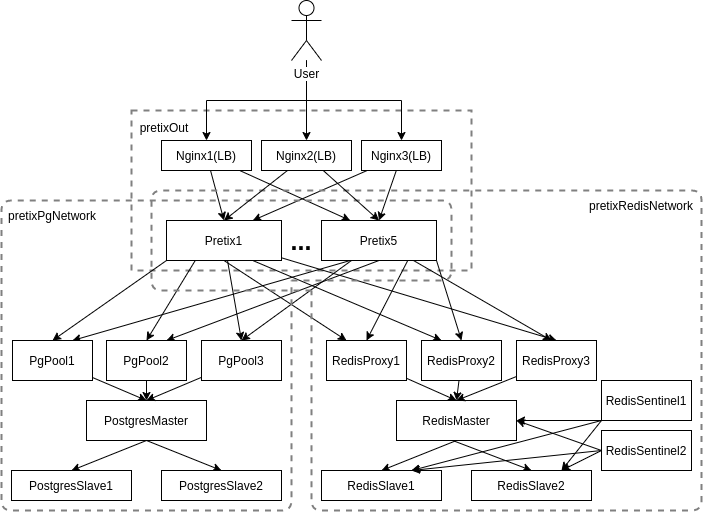
\includegraphics[width=\linewidth]{diagrams/InfrastructureArchitecture.png}
%  \end{minipage}%
%  \caption{Infrastructure architecture diagram deployed in Docker Swarm.}
%  \label{fig:InfrastructureArchitecture}
% \end{figure}

% \begin{figure}[H]
%   \centering
%   \begin{minipage}{\textwidth}
%     \centering
%     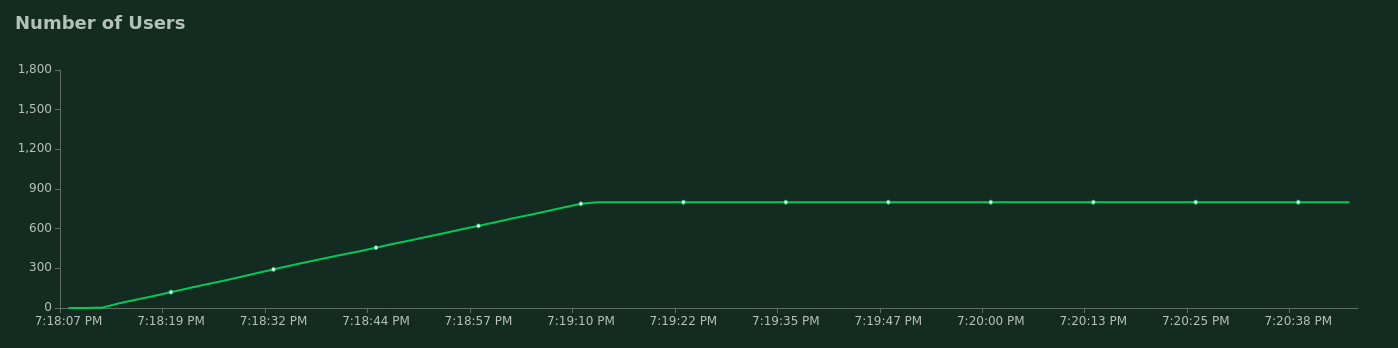
\includegraphics[width=\linewidth]{tests/local/800/number_of_users_1588097887.png}
%   \end{minipage}%
%   \label{fig:LocalTests:number_of_users}
%   \begin{minipage}{\textwidth}
%     \centering
%     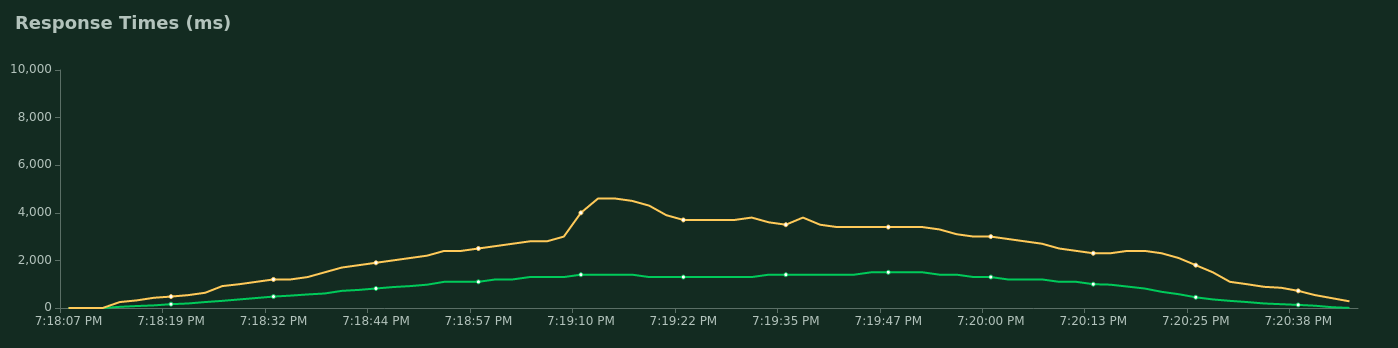
\includegraphics[width=\linewidth]{tests/local/800/response_times_(ms)_1588097887.png}
%   \end{minipage}%
%   \label{fig:LocalTests:response_times_(ms)}
%   \begin{minipage}{\textwidth}
%     \centering
%     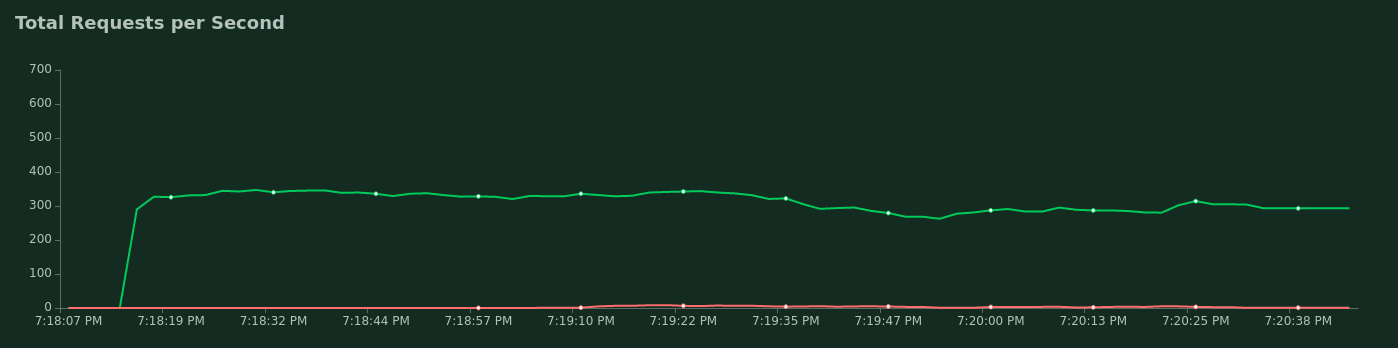
\includegraphics[width=\linewidth]{tests/local/800/total_requests_per_second_1588097887.png}
%   \end{minipage}%
%   \caption{Load tests results with 800 users.}
%   \label{fig:LocalTests:total_requests_per_second}
% \end{figure}
% \vspace{-10pt}

\newpage
\section{System Architecture} \label{architecture} %%%%%%%%%%%%%%%%%%%%%%%%%%%%%%%%%%%%%%%%%%%%%%%%%%%%%%%%%%%%%%%%%%%%%%%%%%%%%%%%%%%%%%%%%%%%%%%%%%%%%%%%%%%%%

\subsection{Infrastructure} \label{architecture.infrastructure} %%%%%%%%%%%%% 

...


\subsection{Redundancy} \label{architecture.redundancy} %%%%%%%%%%%%%%%%%%%%

...

\subsection{Load Balancing} \label{architecture.loadbalancing} %%%%%%%%%%%%%

...

\newpage
\section{Infrastructure Management} \label{management} %%%%%%%%%%%%%%%%%%%%%%%%%%%%%%%%%%%%%%%%%%%%%%%%%%%%%%%%%%%%%%%%%%%%%%%%%%%%%%%%%%%%%%%%%%%%%%%%%%%%%%%%%

\subsection{Service Level Agreements} \label{management.sla} %%%%%%%%%%%%%%%

...

\subsection{Monitoring} \label{management.monitoring} %%%%%%%%%%%%%%%%%%%%%

...

\subsection{Automation} \label{management.automation} %%%%%%%%%%%%%%%%%%%%%

...

\newpage
\section{Quality Assurance} \label{quality} %%%%%%%%%%%%%%%%%%%%%%%%%%%%%%%%%%%%%%%%%%%%%%%%%%%%%%%%%%%%%%%%%%%%%%%%%%%%%%%%%%%%%%%%%%%%%%%%%%%%%%%%%%%%%%%%%%%%

...

\subsection{Scalability} \label{quality.scalability} %%%%%%%%%%%%%%%%%%%%%

...

\subsection{Fault Tolerance} \label{quality.faulttolerance} %%%%%%%%%%%%%%%%%

...

\newpage
\section{Additional Remarks} \label{remarks} %%%%%%%%%%%%%%%%%%%%%%%%%%%%%%%%%%%%%%%%%%%%%%%%%%%%%%%%%%%%%%%%%%%%%%%%%%%%%%%%%%%%%%%%%%%%%%%%%%%%%%%%%%%%%%%%%%%

\subsection{Pretix Quickstart} \label{remarks.quickstart} %%%%%%%%%%%%%%%%%

% quickstart script

During development, a need for a faster basic setup of Pretix emerged for debugging purposes.
As many of our tests assumed the existence of organizers and events already inserted on the databases, each time these had to be cleared the objects had to be 
manually created before proceeding with some implementation process.

In order to respond to this need, we developed a Python script capable of completely dispose of the manual labour.
This script, which we called \texttt{quickstart.py} and placed under a dedicated folder, uses Selenium \cite{selenium} to create an organization inside Pretix, 
generate a secret API key for sending REST requests (storing it in a text file), create a default event and prepare it for load testing with Locust.
It also contains configurable variables to personalize its output.

Such quickstart tool was not only found useful for the obvious advantage in development speed it brought to us, but was also considered a good help tool for any 
person that wishes to quickly experiment our infrastructure without having to know much about Pretix itself.

\subsection{Documentation} \label{remarks.documentation} %%%%%%%%%%%%%%%%

% what documentation was produced?

A great portion of the code we deal with isn't of our authorship, so the documentation it contains is the documentation we get.
Nevertheless, the code we developed has specific purposes and, although usually very much self explanatory due to its nature, should be easy to interpret by any person.
Our goal is to ensure that what we deliver can be easily reused or even continued by other developers.

With this in mind, we made significant efforts on ensuring that all code developed by us followed a common structure with the same coding style.
Also, we made sure all source files have a description of their purpose and relevant information on the first lines, and contain comments on key points of the 
code explaining snippets considered of greater complexity/importance.

\subsection{Assignment Contributions} \label{remarks.contributions} %%%%%%%%%

% who did what?

Regarding the work distribution amongst developers, a close-contact strategy was defined where each worked on a cluster component or piece of software according 
to a predefined plan. 
The cluster strategy and respective details were decided in conjunction, as well as the key objectives and tasks to be achieved before the final delivery deadline.

Pretix' features were explored by both developers in order to better comprehend the web platform and the REST API.
Then, João focused on the deployment of our solution on the department's infrastructure while Filipe focused on creating and executing the load tests.
The analysis of the results were carefully conducted in conjunction as well, in order to maintain a common knowledge for better workflows.
It is needless to say that bug and error solving was made along the development phase by both developers any time it was required.
Once performance benchmarking and bottleneck identification were completed, this report and the code documentation became our primary concern, with both 
contributing equally.

\newpage
\section*{Conclusions} \label{conclusions} %%%%%%%%%%%%%%%%%%%%%%%%%%%%%%%%%%%%%%%%%%%%%%%%%%%%%%%%%%%%%%%%%%%%%%%%%%%%%%%%%%%%%%%%%%%%%%%%%%%%%%%%%%%%%%%%%%%%%

...

\newpage
\begin{thebibliography}{9} %%%%%%%%%%%%%%%%%%%%%%%%%%%%%%%%%%%%%%%%%%%%%%%%%%%%%%%%%%%%%%%%%%%%%%%%%%%%%%%%%%%%%%%%%%%%%%%%%%%%%%%%%%%%%%%%%%%%%%%%%%%%%%%%%%%%%
  \bibliographystyle{Science}

  \bibitem{assign}
    J. P. Barraca,
    \textit{GIC - Report no.2: Simple Product Operation},
    University of Aveiro,
    2019/20.
    \vspace{-10pt}

  \bibitem{pretix}
    \textit{About Pretix},
    \url{https://pretix.eu/about/en/}.
    Pretix.eu,
    retrieved in April 2020.
    \vspace{-10pt}

  \bibitem{rami.io}
    \textit{Welcome to Rami.io},
    \url{https://rami.io/}.
    Rami.io,
    retrieved in April 2020.
    \vspace{-10pt}

  \bibitem{pretixgit}
    \textit{Pretix Code Repository},
    \url{https://github.com/pretix/pretix}.
    GitHub, Inc.,
    retrieved in April 2020.
    \vspace{-10pt}

  \bibitem{pretixdoc}
    \textit{Welcome to pretix' documentation!},
    \url{https://docs.pretix.eu/en/latest/}.
    Pretix.eu,
    retrieved in April 2020.
    \vspace{-10pt}

  \bibitem{docker}
    \textit{Docker Homepage},
    \url{https://www.docker.com/}.
    Docker Inc.,
    retrieved in April 2020.
    \vspace{-26pt}

  \bibitem{pretix_img}
    \textit{pretix/standalone},
    \url{https://hub.docker.com/r/pretix/standalone}.
    pretix,
    retrieved in April 2020.
    \vspace{-10pt}

  \bibitem{django}
    \textit{Meet Django},
    \url{https://www.djangoproject.com/}.
    Django Software Foundation and individual contributors,
    retrieved in April 2020.
    \vspace{-10pt}

  \bibitem{gunicorn}
    \textit{Gunicorn Homepage},
    \url{https://gunicorn.org/}.
    Gunicorn.org,
    retrieved in April 2020.
    \vspace{-10pt}

  \bibitem{nginx}
    \textit{NGinX News},
    \url{https://nginx.org/}.
    NGinX.org,
    retrieved in April 2020.
    \vspace{-10pt}

  \bibitem{postgresql}
    \textit{PostgreSQL: The World's Most Advanced Open Source Relational Database},
    \url{https://www.postgresql.org/}.
    The PostgreSQL Global Development Group,
    retrieved in April 2020.
    \vspace{-10pt}

  \bibitem{redis}
    \textit{About Redis},
    \url{https://redis.io/}.
    Redis Labs,
    retrieved in April 2020.
    \vspace{-10pt}

  \bibitem{pgpool}
    \textit{Welcome to Pgpool-II},
    \url{https://www.pgpool.net/mediawiki/index.php/Main_Page}.
    PgPool Global Development Group,
    retrieved in April 2020.
    \vspace{-10pt}

  \bibitem{haproxy}
    \textit{HAProxy: The Reliable, High Performance TCP/HTTP Load Balancer},
    \url{https://www.haproxy.org/}.
    HAProxy.org,
    retrieved in April 2020.
    \vspace{-10pt}

  \bibitem{locust}
    \textit{Locust, an open source load testing tool},
    \url{https://locust.io/}.
    Locust.io,
    retrieved in April 2020.
    \vspace{-10pt}

  \bibitem{selenium}
    \textit{About Selenium},
    \url{https://www.selenium.dev/about/}.
    Software Freedom Conservancy,
    retrieved in April 2020.
    \vspace{-10pt}

  \bibitem{ansible}
    \textit{Ansible},
    \url{https://www.ansible.com/}.
    Red Hat,
    retrieved in April 2020.
    
\end{thebibliography}

\clearpage

\end{document}




















